\documentclass[11pt,a4paper]{article}

\usepackage[brazil]{babel}
\usepackage[T1]{fontenc}
\usepackage{lmodern}
\usepackage{microtype}
\usepackage[margin=2.2cm]{geometry}
\usepackage{amsmath}
\usepackage{booktabs}
\usepackage{tabularx}
\usepackage{enumitem}
\usepackage{graphicx}
\usepackage{float}
\usepackage{caption}
\usepackage[hidelinks]{hyperref}

\setlist{nosep, leftmargin=*}
\setlength{\parskip}{0.4em}
\setlength{\parindent}{0pt}
\captionsetup{font=small, labelfont=bf}
\graphicspath{{figuras/}}

\title{\textbf{Q-learning no Lago Congelado com taxa de aprendizado decrescente}\\[0.3em]
  \large Relatório de experimentos}
\author{Luisa Ferreira\\
  \small Inteligência Artificial para Jogos I --- Aprendizado por Reforço}
\date{Novembro de 2026}

\begin{document}
\maketitle

\textbf{Código:} o notebook com a implementação, os experimentos e todas as saídas é o arquivo
\texttt{qlearning\_toy\_text\_luisa.ipynb}, e o agente está em \texttt{agente\_luisa.py}, disponíveis em:\\
\url{https://github.com/ctrindadedev/game-ai-lab/tree/master/QLearningToyText/luisa}

O código foi desenvolvido no mesmo repositório do colega Caio Trindade. Esta versão parte de uma cópia do notebook dele
(mesmo agente da disciplina e mesmo protocolo de avaliação), mas estuda um eixo que ele não explorou: \textbf{a taxa
de aprendizado $\alpha$ deixar de ser constante e diminuir ao longo do treino}. Os mapas e as métricas também são
outros.

O agente é o do notebook disponibilizado na disciplina: uma Q-table atualizada por diferença temporal,
\[
Q(s,a) \leftarrow Q(s,a) + \alpha_t\left[r + \gamma \max_{a'} Q(s',a') - Q(s,a)\right],
\]
com política $\varepsilon$-greedy e decaimento linear de $\varepsilon$. A única mudança é de onde vem $\alpha_t$.
A motivação é teórica: o Q-learning só converge para $Q^*$ se a taxa de cada par $(s,a)$ satisfizer as condições de
Robbins-Monro, $\sum_t \alpha_t = \infty$ e $\sum_t \alpha_t^2 < \infty$. Com $\alpha$ constante a segunda condição falha, e
num ambiente estocástico a Q-table fica oscilando em torno do valor certo. A pergunta é se isso aparece na prática, em
20000 episódios, e qual ritmo de decaimento funciona.

\section{Ambientes}

\subsection*{FrozenLake-v1 (Lago Congelado)}

\begin{itemize}
  \item \textbf{Estados:} a célula do grid, $\text{linha} \times 8 + \text{coluna}$ (64 estados nos mapas 8x8).
  \item \textbf{Ações:} 4 (esquerda, baixo, direita, cima).
  \item \textbf{Reforço:} $+1$ ao chegar no objetivo \texttt{G} e $0$ em qualquer outro passo, inclusive ao cair num
    buraco \texttt{H}, que encerra o episódio. O limite é de 100 passos.
  \item \textbf{Escorregadio} (\texttt{is\_slippery=True}): o agente só vai na direção escolhida com probabilidade
    $1/3$; nas outras vezes desliza para uma das direções perpendiculares.
  \item \textbf{Desafios:} a recompensa é esparsa (até o agente chegar ao objetivo por acaso, a Q-table fica toda
    zerada). No gelo escorregadio o alvo $r + \gamma\max_{a'}Q(s',a')$ de um mesmo par $(s,a)$ muda de uma visita para
    outra, porque o estado seguinte é sorteado. É esse ruído que torna a escolha de $\alpha$ importante.
\end{itemize}

Foram usados dois mapas 8x8, ambos diferentes dos do colega. O principal é o \textbf{mapa padrão do Gymnasium}
(\texttt{FrozenLake8x8-v1}), com 10 buracos, usado na versão determinística (como controle) e na escorregadia. O segundo é
um \textbf{mapa aleatório com $p = 0{,}8$} (\texttt{generate\_random\_map(size=8, p=0.8, seed=9)}), em que $p$ é a
probabilidade de uma célula ser gelo; ele tem 13 buracos e foi usado só na versão escorregadia, para verificar se os
resultados se repetem. Nos dois, o menor caminho tem 14 passos.

\begin{center}
\footnotesize
\renewcommand{\arraystretch}{0.8}
\begin{tabular}{cc}
\texttt{SFFFFFFF} & \texttt{SFFFFHHH}\\
\texttt{FFFFFFFF} & \texttt{FFFFFHHF}\\
\texttt{FFFHFFFF} & \texttt{FFFFFFHH}\\
\texttt{FFFFFHFF} & \texttt{HHFFHFFF}\\
\texttt{FFFHFFFF} & \texttt{FFFFFHFF}\\
\texttt{FHHFFFHF} & \texttt{FFFFHFFF}\\
\texttt{FHFFHFHF} & \texttt{FFFFFFHF}\\
\texttt{FFFHFFFG} & \texttt{FFFFFFFG}\\[0.3em]
8x8 padrão & 8x8 $p = 0{,}8$ (semente 9)
\end{tabular}
\end{center}

Duas referências exatas foram calculadas por programação dinâmica sobre o modelo do próprio ambiente
(\texttt{env.unwrapped.P}):
\begin{itemize}
  \item \textbf{Sucesso máximo:} a maior probabilidade de chegar ao \texttt{G} em até 100 passos. É \textbf{0,641} no
    mapa padrão escorregadio e \textbf{0,597} no mapa $p = 0{,}8$ escorregadio (1,0 nos determinísticos).
  \item \textbf{$Q^*$:} o ponto fixo para o qual o Q-learning com $\gamma = 0{,}95$ deve convergir, obtido por iteração de
    valor. Com ele dá para medir diretamente o erro da Q-table aprendida, o que não depende de rodar episódios de teste.
\end{itemize}

\section{Metodologia experimental}

\subsection{Configuração dos experimentos}

Tudo o que não é $\alpha$ fica igual à configuração base do notebook original:

\begin{center}
\small
\begin{tabular}{ll}
\toprule
Parâmetro & Valor \\
\midrule
Fator de desconto $\gamma$ & 0,95 \\
$\varepsilon$ ($\varepsilon$-greedy) & de 0,5 até 0,1, decaimento linear ao longo do treino \\
Q-table inicial & zeros \\
Episódios de treino & 5000 no determinístico, 20000 no escorregadio \\
Repetições & 5 sementes (0 a 4) por configuração \\
\bottomrule
\end{tabular}
\end{center}

Foram comparadas oito programações de $\alpha$, sendo $N(s,a)$ o número de atualizações já feitas no par:

\begin{center}
\small
\begin{tabular}{lll}
\toprule
Programação & Fórmula & Ideia \\
\midrule
$\alpha = 0{,}5$ (base) & constante & o notebook original \\
$\alpha = 0{,}1$ & constante & o melhor $\alpha$ do colega no gelo escorregadio \\
$\alpha = 0{,}02$ & constante & pequeno desde o início \\
$1/(1+N)$ & $\alpha_t(s,a) = 1/(1+N(s,a))$ & média simples dos alvos do par \\
$1/(1+N)^{0,8}$ & $\alpha_t(s,a) = 1/(1+N(s,a))^{0,8}$ & decai mais devagar \\
$1/(1+N)^{0,6}$ & $\alpha_t(s,a) = 1/(1+N(s,a))^{0,6}$ & decai ainda mais devagar \\
$\max(0{,}05;\ 1/(1+N))$ & a média simples, com piso & nunca para de aprender \\
linear $0{,}5 \to 0{,}01$ & $\alpha_t = 0{,}5 - 0{,}49 \cdot \text{episódio}/\text{total}$ & uma taxa global, igual para todos os pares \\
\bottomrule
\end{tabular}
\end{center}

As programações por visitas com $0{,}5 < \omega \le 1$ satisfazem as condições de Robbins-Monro; as constantes e a com
piso, não; a linear por episódio chega a um valor fixo no fim do treino. A Figura~\ref{fig:programacoes} mostra como cada
programação por visitas cai.

\begin{figure}[H]
  \centering
  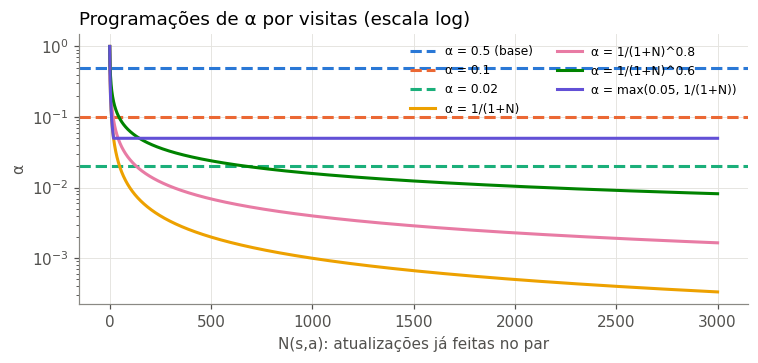
\includegraphics[width=0.7\textwidth]{exp0_programacoes_alpha.png}
  \caption{Programações de $\alpha$ em função do número de atualizações do par (escala log).}
  \label{fig:programacoes}
\end{figure}

\begin{itemize}
  \item \textbf{Experimento 1:} as oito programações no 8x8 padrão determinístico (controle, sem ruído de transição).
  \item \textbf{Experimento 2:} as oito programações no 8x8 padrão escorregadio.
  \item \textbf{Experimento 3:} as oito programações no 8x8 $p = 0{,}8$ escorregadio.
  \item \textbf{Experimento 4:} comparação das políticas aprendidas com a política ótima e contagem de atualizações por
    estado.
\end{itemize}

\textbf{Hipóteses iniciais.}
(H1) No ambiente determinístico, a programação de $\alpha$ não deve mudar a política final.
(H2) No escorregadio, $\alpha$ constante e alto deve deixar a política instável até o fim do treino.
(H3) $\alpha$ decrescente deve dar uma Q-table mais próxima de $Q^*$ e uma política melhor que qualquer $\alpha$
constante.
(H4) $\alpha = 1/(1+N)$, a média simples, deve ser a melhor das programações decrescentes, por ser a estimativa
``natural'' de uma média.

\textbf{Critério de parada:} número fixo de episódios. Cada episódio termina num estado terminal ou no limite de 100
passos. \textbf{Ferramentas:} Python 3.12, Gymnasium 1.4, NumPy, pandas e Matplotlib, num notebook Jupyter. O agente fica
num módulo separado para que as 120 execuções (8 programações $\times$ 3 ambientes $\times$ 5 sementes) rodem em paralelo;
cada execução usa só a própria semente, então o resultado não depende do paralelismo.

\subsection{Procedimentos de treinamento e avaliação}

Em cada episódio de treino o agente escolhe ações com $\varepsilon$-greedy e atualiza a Q-table a cada passo, usando o
$\alpha$ da programação. A cada 25 episódios, a política gulosa ($\varepsilon = 0$, sem atualizar a tabela) joga 20
episódios; ao fim do treino, mais 500 para a avaliação final. Além disso, a cada teste foram registradas:

\begin{itemize}
  \item \textbf{Erro contra $Q^*$:} a média de $|Q(s,a) - Q^*(s,a)|$ nos estados não terminais. Mede se a tabela
    convergiu.
  \item \textbf{Trocas de ação:} em quantos estados a ação gulosa mudou desde o teste anterior. Mede se a política
    estabilizou. Uma tabela pode parar de mudar sem ter convergido, e as duas medidas juntas separam os dois casos.
  \item \textbf{$\alpha$ médio:} a média dos $\alpha$ efetivamente usados nas atualizações.
\end{itemize}

As tabelas trazem o \textbf{sucesso final} (média $\pm$ desvio padrão entre as sementes) e em \% do sucesso máximo; o
\textbf{teste médio} (média de todos os testes gulosos do treino, que resume a velocidade de aprendizado); o primeiro
episódio em que o teste guloso atingiu 40\% de sucesso (cerca de dois terços do máximo); e o \textbf{acordo com
$\pi^*$}, a fração dos estados em que a ação gulosa final é uma ação ótima segundo $Q^*$.

\section{Resultados}

\subsection*{Controle: 8x8 determinístico}

As oito programações chegaram a $1{,}000 \pm 0{,}000$ de sucesso, todas passando de 90\% no mesmo episódio (1010), com
curvas de teste idênticas. O erro final contra $Q^*$, porém, variou: 0,18 com $\alpha = 0{,}5$ e 0,46 com $1/(1+N)$.

\subsection*{8x8 padrão escorregadio}

\begin{table}[H]
\centering
\footnotesize\setlength{\tabcolsep}{4pt}
\caption{8x8 padrão escorregadio, 20000 episódios (média $\pm$ desvio padrão entre 5 sementes). Sucesso máximo: 0,641.
``Trocas'' é a média de estados que mudaram de ação gulosa por teste no último quinto do treino.}
\label{tab:padrao}
\begin{tabular}{lcccccc}
\toprule
Programação de $\alpha$ & Sucesso final & \% do máx. & Teste médio & Ep. até 40\% & Erro $|Q-Q^*|$ & Trocas \\
\midrule
0,5 (base)              & $0{,}221 \pm 0{,}127$ & 34 & 0,191 & 1620 (5/5) & 0,0400 & 16,5 \\
0,1                     & $0{,}512 \pm 0{,}082$ & 80 & 0,428 & 1640 (5/5) & 0,0206 & 5,9 \\
0,02                    & $0{,}542 \pm 0{,}035$ & 85 & 0,395 & 5455 (5/5) & 0,0266 & 1,3 \\
$1/(1+N)$               & $0{,}182 \pm 0{,}093$ & 28 & 0,135 & 6583 (3/5) & 0,0693 & 0,0 \\
$1/(1+N)^{0,8}$         & $0{,}377 \pm 0{,}075$ & 59 & 0,295 & 3760 (5/5) & 0,0375 & 0,1 \\
$1/(1+N)^{0,6}$         & $\mathbf{0{,}588 \pm 0{,}022}$ & \textbf{92} & \textbf{0,534} & 1505 (5/5) & \textbf{0,0072} & 0,3 \\
$\max(0{,}05;\ 1/(1+N))$ & $0{,}553 \pm 0{,}062$ & 86 & 0,480 & 1740 (5/5) & 0,0118 & 3,6 \\
linear $0{,}5 \to 0{,}01$ & $\mathbf{0{,}593 \pm 0{,}016}$ & \textbf{93} & 0,334 & 1365 (5/5) & 0,0111 & 3,9 \\
\bottomrule
\end{tabular}
\end{table}

\begin{figure}[H]
  \centering
  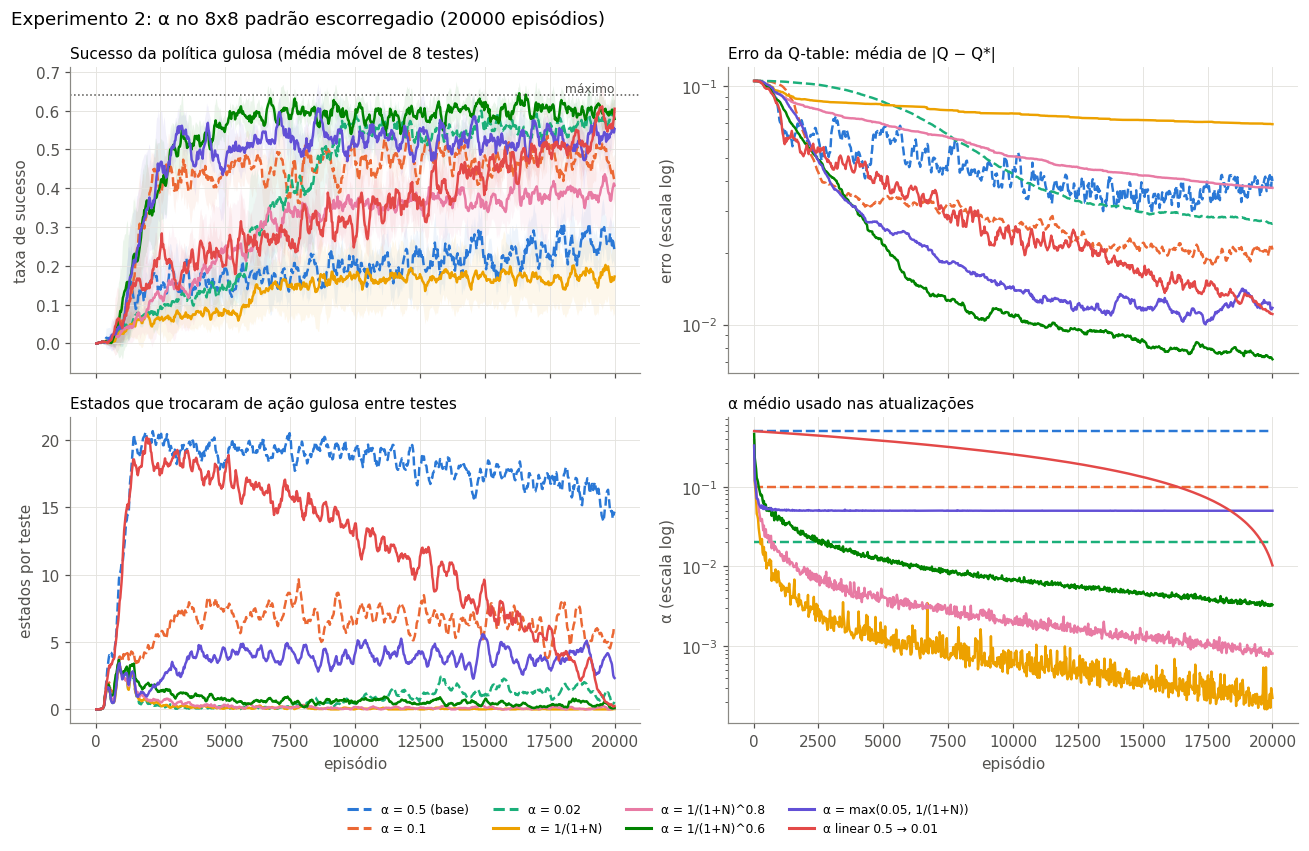
\includegraphics[width=\textwidth]{exp2_escorregadio_padrao.png}
  \caption{8x8 padrão escorregadio. Linhas tracejadas: $\alpha$ constante; linhas cheias: $\alpha$ decrescente. Curvas
    são a média de 5 sementes.}
  \label{fig:padrao}
\end{figure}

Com $\alpha = 0{,}5$ a política gulosa trocou de ação em 15 a 20 estados a cada teste do começo ao fim, e o sucesso
ficou em torno de 0,2 (Figura~\ref{fig:padrao}). Entre os constantes, reduzir $\alpha$ ajudou: 0,1 e 0,02 chegaram a
80\% e 85\% do máximo, mas com 0,02 o teste só passou de 40\% por volta do episódio 5455. A média simples
$1/(1+N)$ foi a \textbf{pior} configuração: o $\alpha$ efetivo caiu para cerca de $10^{-3}$ em 2500 episódios, a
política parou de mudar (0,0 trocas) e o erro contra $Q^*$ ficou o maior de todos. $1/(1+N)^{0,6}$ teve o melhor teste
médio, o menor erro contra $Q^*$ (5,6 vezes menor que a base) e quase nenhuma troca no fim. O decaimento linear chegou
ao mesmo sucesso final, mas passou boa parte do treino oscilando como $\alpha = 0{,}5$.

\subsection*{8x8 $p = 0{,}8$ escorregadio}

\begin{table}[H]
\centering
\footnotesize\setlength{\tabcolsep}{4pt}
\caption{8x8 $p = 0{,}8$ escorregadio, 20000 episódios. Sucesso máximo: 0,597.}
\label{tab:p08}
\begin{tabular}{lcccccc}
\toprule
Programação de $\alpha$ & Sucesso final & \% do máx. & Teste médio & Ep. até 40\% & Erro $|Q-Q^*|$ & Trocas \\
\midrule
0,5 (base)              & $0{,}250 \pm 0{,}138$ & 42 & 0,144 & 3585 (5/5) & 0,0466 & 15,6 \\
0,1                     & $0{,}447 \pm 0{,}054$ & 75 & 0,336 & 3880 (5/5) & 0,0299 & 6,0 \\
0,02                    & $0{,}390 \pm 0{,}169$ & 65 & 0,138 & 13481 (4/5) & 0,0791 & 0,3 \\
$1/(1+N)$               & $0{,}065 \pm 0{,}046$ & 11 & 0,049 & 9375 (1/5) & 0,1029 & 0,0 \\
$1/(1+N)^{0,8}$         & $0{,}217 \pm 0{,}147$ & 36 & 0,136 & 9475 (3/5) & 0,0618 & 0,0 \\
$1/(1+N)^{0,6}$         & $\mathbf{0{,}550 \pm 0{,}030}$ & \textbf{92} & \textbf{0,391} & 4905 (5/5) & \textbf{0,0106} & 0,4 \\
$\max(0{,}05;\ 1/(1+N))$ & $0{,}465 \pm 0{,}089$ & 78 & 0,369 & 4005 (5/5) & 0,0212 & 3,6 \\
linear $0{,}5 \to 0{,}01$ & $\mathbf{0{,}561 \pm 0{,}026}$ & \textbf{94} & 0,276 & 3385 (5/5) & 0,0153 & 4,3 \\
\bottomrule
\end{tabular}
\end{table}

A ordem se repetiu no segundo mapa (Tabela~\ref{tab:p08}, Figura~\ref{fig:p08}). As diferenças com o mapa padrão foram
o $\alpha = 0{,}02$ constante, que piorou bastante (65\%, com uma semente sem chegar a 40\%), e o $1/(1+N)$, que caiu
para 11\% do máximo.

\begin{figure}[H]
  \centering
  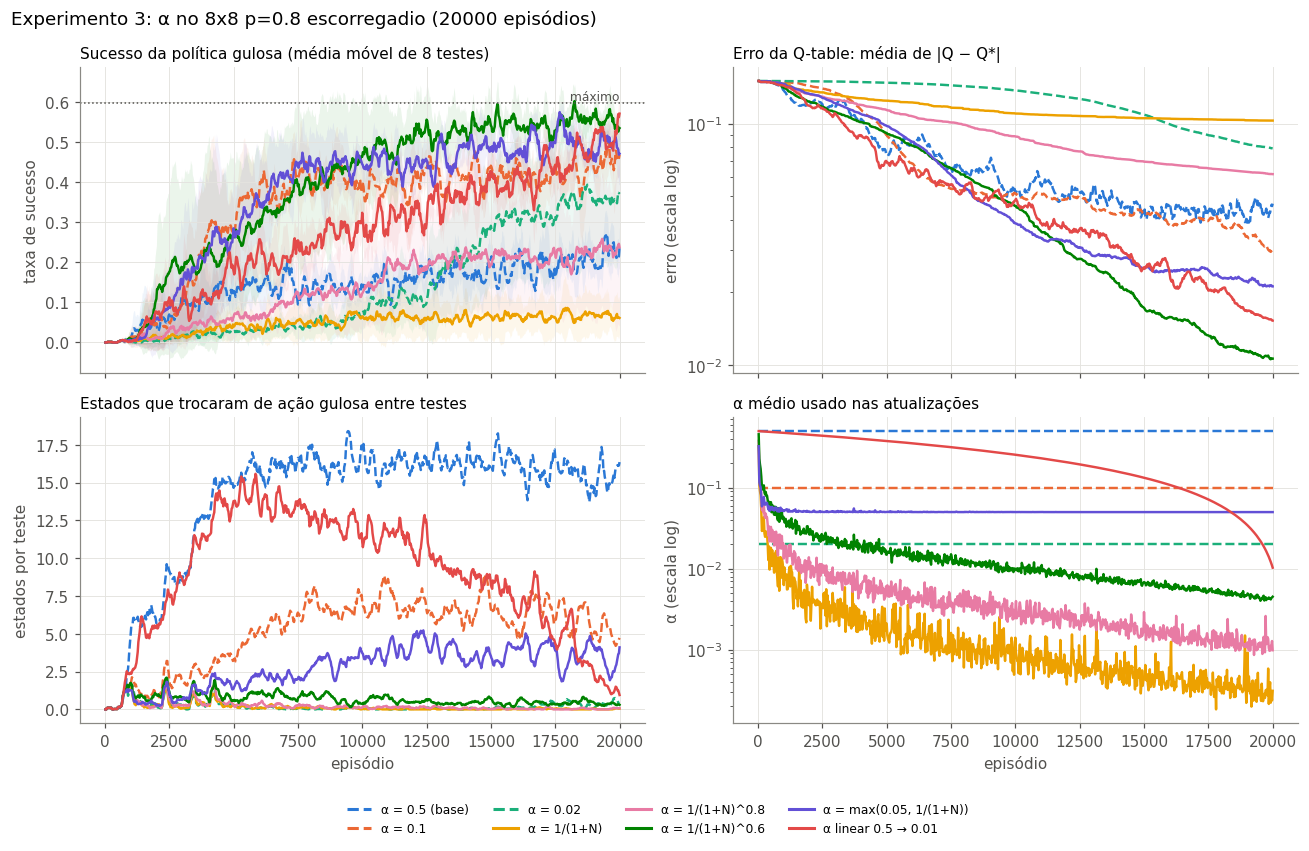
\includegraphics[width=\textwidth]{exp3_escorregadio_p08.png}
  \caption{8x8 $p = 0{,}8$ escorregadio.}
  \label{fig:p08}
\end{figure}

\subsection*{Análise qualitativa}

A Figura~\ref{fig:politicas} compara a política gulosa final (semente 0) da base, do melhor $\alpha$ constante e da
melhor programação decrescente com a política ótima. A base erra a ação em vários estados, inclusive perto do objetivo; a
política com $\alpha$ decrescente coincide com a ótima em quase todo o mapa. A política ótima no gelo escorregadio é
pouco intuitiva: perto dos buracos ela aponta ``para longe'' deles, contando que, se escorregar, o deslize é para os
lados e não para dentro do buraco.

\begin{figure}[H]
  \centering
  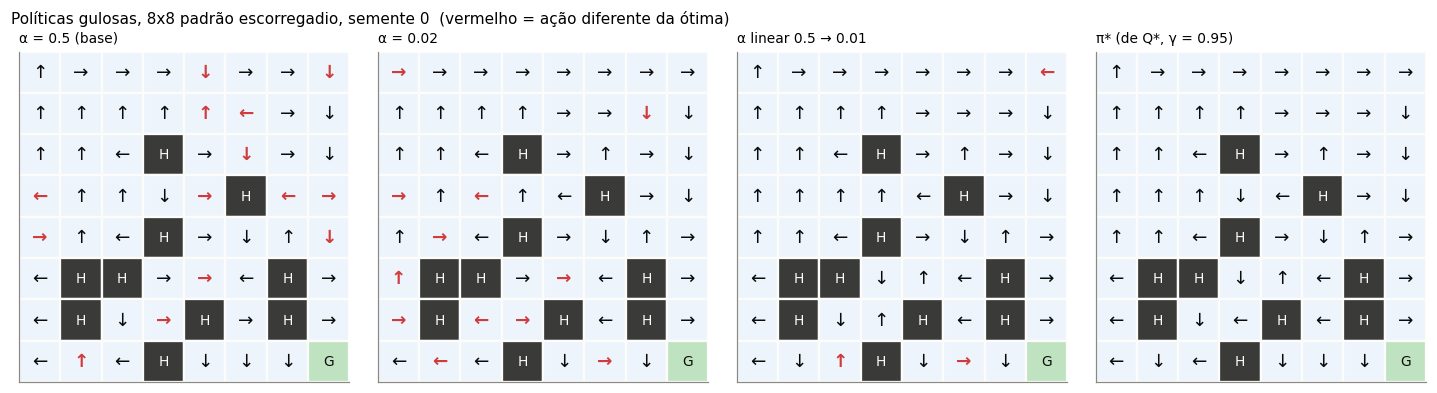
\includegraphics[width=\textwidth]{exp4_politicas.png}
  \caption{Políticas gulosas finais no 8x8 padrão escorregadio (semente 0). Setas vermelhas: ação diferente da ótima
    segundo $Q^*$.}
  \label{fig:politicas}
\end{figure}

A Figura~\ref{fig:visitas} mostra quantas atualizações cada estado recebeu: o estado inicial, cerca de $10^5$; os do
fundo do mapa, perto do objetivo, menos de 100.

\begin{figure}[H]
  \centering
  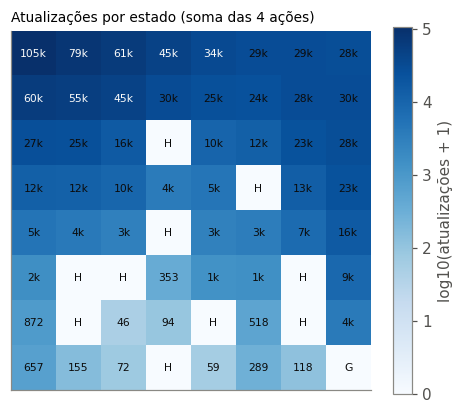
\includegraphics[width=0.45\textwidth]{exp4_visitas.png}
  \caption{Atualizações por estado (soma das quatro ações), média das sementes, configuração base, 8x8 padrão
    escorregadio.}
  \label{fig:visitas}
\end{figure}

\section{Discussão}

\textbf{H1 foi confirmada.} No determinístico, até o agente achar o objetivo a Q-table é toda zero e, depois disso,
qualquer $\alpha > 0$ deixa positivas as mesmas ações. Com as mesmas sementes, o agente toma as mesmas decisões, o que
explica o episódio 1010 repetido (o colega observou o mesmo efeito com $\alpha$ e $\gamma$ constantes). Sem ruído de
transição não há o que $\alpha$ decrescente corrigir; pelo contrário, um $\alpha$ que cai depressa deixa o valor do
objetivo se propagar mais devagar até o início do mapa, o que explica o erro maior contra $Q^*$ de $1/(1+N)$.

\textbf{H2 foi confirmada.} Com $\alpha = 0{,}5$ cada escorregão reescreve metade do valor do par, e a política não
parou de mudar em 20000 episódios. O desvio padrão entre sementes ($\pm 0{,}13$) é outro sinal disso: o resultado final
depende de em que momento da oscilação o treino parou.

\textbf{H3 foi confirmada em parte.} A melhor programação decrescente ($1/(1+N)^{0,6}$) superou todos os $\alpha$
constantes em sucesso, erro contra $Q^*$ e estabilidade, nos dois mapas. Mas não é qualquer decaimento que ajuda:
$1/(1+N)$ e $1/(1+N)^{0,8}$ ficaram abaixo de $\alpha = 0{,}1$ constante.

\textbf{H4 foi refutada.} A média simples foi a pior configuração dos dois mapas. O motivo é que no Q-learning os alvos
não são amostras de uma distribuição fixa: eles usam $\max_{a'} Q(s',a')$, que ainda está sendo aprendido. Os primeiros
alvos foram calculados com a tabela zerada e, na média simples, pesam tanto quanto os últimos. Como os pares perto do
início recebem dezenas de milhares de atualizações (Figura~\ref{fig:visitas}), o $\alpha$ deles chega a $10^{-4}$ ou
menos, e a tabela congela antes que o valor do objetivo chegue até lá. As trocas de ação caem a zero, mas o erro contra
$Q^*$ é o maior: \textbf{a política parou de mudar sem ter convergido}. Isso bate com a análise de Even-Dar e Mansour
(2003, \emph{Learning Rates for Q-learning}): com taxa $1/N$, o número de passos para convergir pode crescer
exponencialmente em $1/(1-\gamma)$, enquanto com taxa polinomial $1/N^{\omega}$, $1/2 < \omega < 1$, o crescimento é
polinomial. Com $\gamma = 0{,}95$, $1/(1-\gamma) = 20$, e o efeito fica visível. Quanto menor o $\omega$ testado, melhor
o resultado.

Duas outras comparações ajudam a entender o resultado:
\begin{itemize}
  \item \textbf{Taxa por par contra taxa global.} O decaimento linear por episódio teve sucesso final equivalente ao de
    $1/(1+N)^{0,6}$, mas um teste médio bem menor (0,33 contra 0,53 no mapa padrão), porque usa $\alpha$ alto por muito
    tempo. Ele também trata igual o estado inicial, com $10^5$ atualizações, e o fundo do mapa, com menos de 100; e
    depende de saber de antemão quantos episódios o treino terá. A taxa por visitas dá passo grande onde há pouca
    informação e passo pequeno onde há muita, sem precisar dessa informação.
  \item \textbf{O piso.} $\max(0{,}05;\ 1/(1+N))$ corrigiu o congelamento da média simples (de 28\% para 86\% no mapa
    padrão), mas a política continuou trocando de ação em cerca de 3,6 estados por teste: com $\alpha$ fixo em 0,05 no
    fim, ela se comporta como um $\alpha$ constante pequeno.
\end{itemize}

\textbf{Limitações.} Foram só 5 sementes por configuração e 20000 episódios; com mais episódios, as programações que
decaem rápido poderiam se recuperar (a teoria garante que elas convergem, só que devagar). $\gamma$ e a exploração
ficaram fixos, e só foram testados três valores de $\omega$. O $Q^*$ é o do problema descontado com $\gamma = 0{,}95$,
cuja política ótima não é exatamente a de maior taxa de sucesso; por isso nenhuma configuração chegaria a 100\% do
sucesso máximo mesmo com a tabela perfeita.

\textbf{Melhorias possíveis:} testar mais valores de $\omega$ (entre 0,5 e 0,7) e combiná-los com um piso; usar a
contagem de visitas também na exploração (por exemplo, $\varepsilon$ por estado); repetir com $\gamma = 0{,}99$, em que a
dependência em $1/(1-\gamma)$ deve tornar a média simples ainda pior; e comparar com o Double Q-learning, que ataca outro
problema do Q-learning em ambientes estocásticos, o viés do $\max$.

\section{Conclusões}

O Q-learning resolveu o FrozenLake determinístico com qualquer programação de $\alpha$. No gelo escorregadio,
$\alpha$ decidiu o resultado: a configuração base ficou em 34--42\% do sucesso máximo, e a taxa de aprendizado
decrescente por visitas $1/(1+N(s,a))^{0,6}$ chegou a 92\% nos dois mapas, com a Q-table mais próxima de $Q^*$ e a
política estável no fim do treino.

As principais lições foram:
\begin{itemize}
  \item em ambientes estocásticos, diminuir $\alpha$ ao longo do treino estabiliza a Q-table, como a teoria prevê, mas o
    ritmo do decaimento importa mais do que decair ou não: a média simples $1/(1+N)$, que parece a escolha natural, foi
    pior que $\alpha$ constante;
  \item uma taxa por par $(s,a)$ funciona melhor que uma taxa global, porque os estados são visitados em quantidades
    muito diferentes;
  \item medir só a taxa de sucesso esconde o que está acontecendo: comparar a Q-table com $Q^*$ e contar as trocas de
    ação separa uma tabela que convergiu de uma que só parou de mudar.
\end{itemize}

\end{document}
